\chap{MLton}{mlton}

This chapter describes the compiler proper, which is found in the {\tt mlton}
directory.

\section{Sources}

\begin{description}

\place{ast}
Abstract syntax trees produced by the front end.

\place{atoms}
Common atomic pieces of syntax trees used throughout the compiler, like
constants, primitives, variables, and types.

\place{backend}
The backend translates from the {\tt Cps} IL to a machine independent IL called
{\tt Machine}.  It decides data representations, stack frame layouts, and creates
runtime system information like limit checks and bitmasks.

\place{call-main.sml}
A one-line file that is the last line of the compiler sources.  It calls the
main function.

\place{closure-convert}
The closure converter, which converts from {\tt Sxml}, the higher-order
simply-typed IL, to {\tt Cps}, the first-order simply-typed IL.

\place{cm}
Support for {\smlnj}-style compilation manager (CM) files.

\place{codegen}
Both the C and the native X86 code generator.

\place{control}
Compiler switches used throughout the rest of the compiler.

\place{core-ml}
The implicitly typed IL that results from defunctorization.  Contains a
pass of dead code elimination for eliminating basis library code.  Also contains
the pass that replaces constants defined by {\tt \_prim} with their values.

\place{elaborate}
The elaborator, which matches variable uses with bindings in the AST IL and
defunctorizes to produce a {\tt CoreML} program.  It does not do type checking
yet, but will someday. 

\place{front-end}
The lexer and parser, which turn files into ASTs.

\place{main}
The two main structures in the compiler, one ({\tt Main}) for handling all the
command line switches and one ({\tt Compile}) which is a high-level view of the
the compiler passes, from front end to code generation.

\place{Makefile}
To make the compiler.

\place{mlton.cm}
An automatically generated file ({\tt make mlton.cm}) that lists all of the
files (in order) that make up the compiler.

\place{mlton.sml}
An automatically generated file ({\tt make mlton.sml}) that contains all of the
compiler sources concatenated together.

\place{rcps}
An experimental IL, similar to CPS, but with more expressive types for
describing representations (hence the ``r'').  Not yet in use.

\place{sources.cm}
For compiling with {\smlnj}.

\place{ssa}
Static-Single-Assignment form, the first-order simply-typed IL on which most
optimization is performed.  There are roughly 20 different optimization passes
(some of which run several times).

\place{type-inference}
The type inference pass, which translates from {\tt CoreML} to {\tt Xml}.

\place{xml}
The {\tt Xml} and {\tt Sxml} intermediate languages.  Also, the passes that
monomorphise, do polvariance, and implement exceptions.

\end{description}

\section{Compiler Overview}

\figref{structure} shows the overall structure of the compiler.  Intermediate
languages (ILs) are shown in ovals.  The names of compiler passes adorn arrows
between ILs.  In this section I give a brief description of each pass and a
pointer to a later section that covers the pass in detail.  Each IL also has a
separate section devoted to it.
\figBegin
\centerline{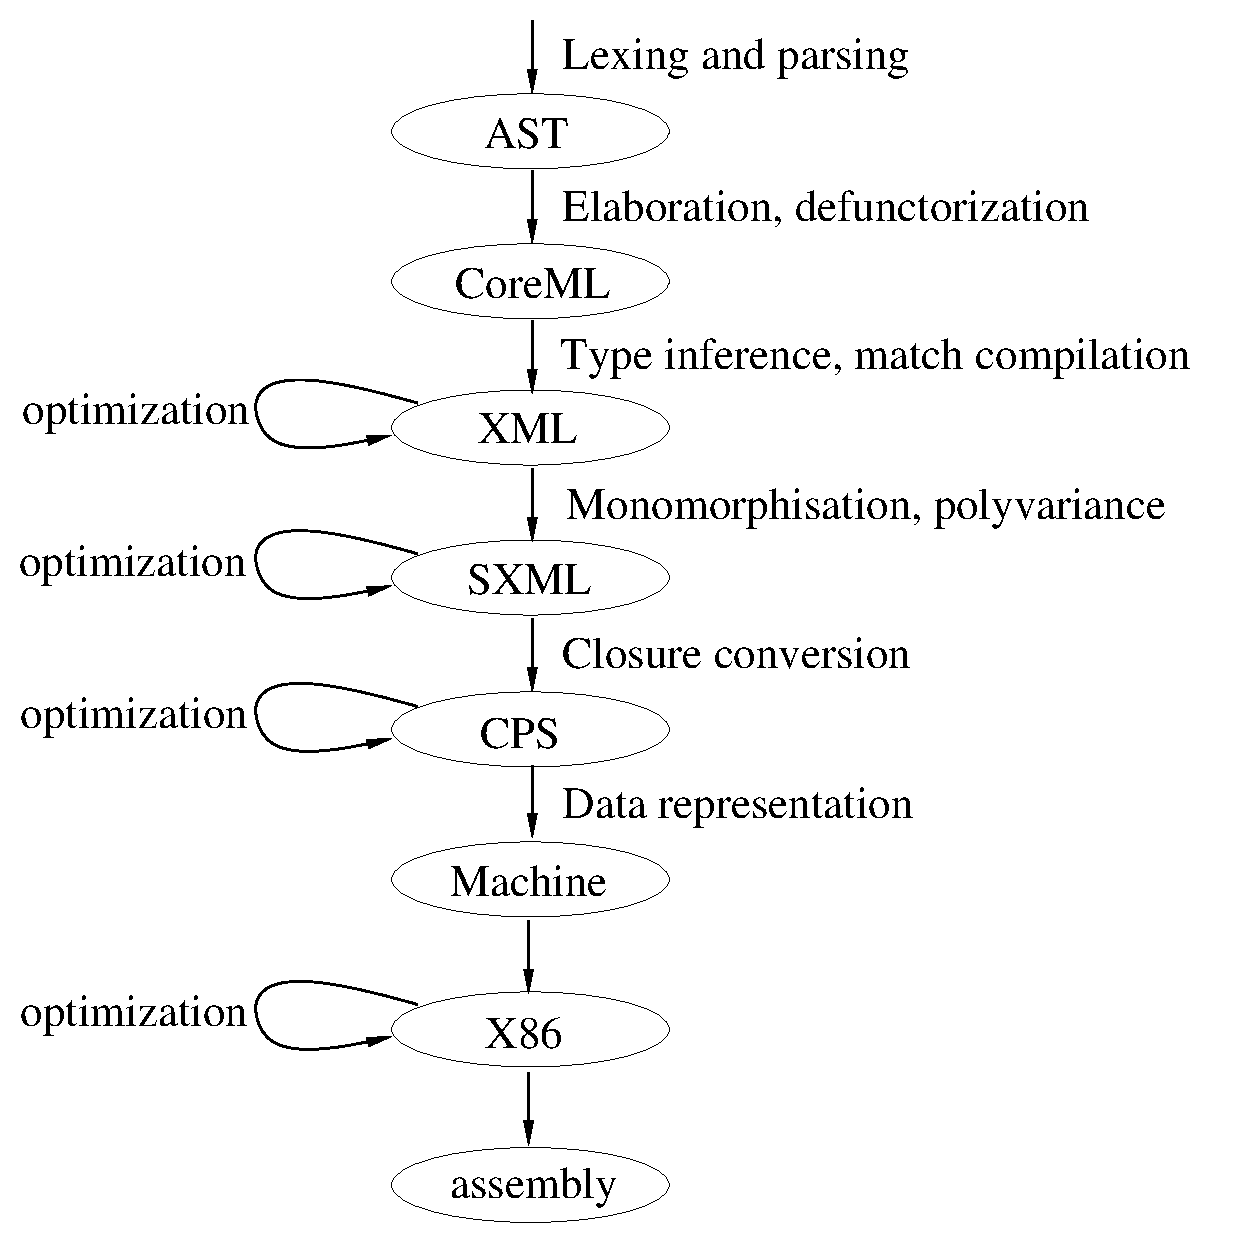
\epsfig{file=structure.eps,width=5.0in}}
\figEnd{Compiler structure}
       {structure}

The front end (\chapref{front-end}) takes SML source code (a complete
program) and performs lexing and parsing, producing an abstract syntax
tree (\chapref{ast}).  The lexer is produced by
ml-lex\cite{AppelEtAl94} and the parser is produced by
ml-yacc\cite{TarditiAppel94}.  The specifications for 
the lexer and parser were originally taken from \smlnj 109.32.  The
lexer is unchanged.  I have substantially modified the actions in the
grammar to produce my own version of abstract syntax trees (similar
to, but different from {\smlnj}).

Defunctorization (\chapref{defunctorization}), translates abstract
syntax trees to a small implicitly typed core language, called Core ML
(\chapref{core-ml}).  Its primary task is to eliminate all uses of the
module system (signatures, structures, functors).  It does this by
applying all functors and flattening all structures, moving
declarations to the top level.  This phase also performs precedence
parsing of infix expressions and patterns (the code to do this was
taken from \smlnj).  Finally, it does some amount of "macro
expansion", so that the core language is smaller.

Type inference (\chapref{type-inference}) translates implicitly typed
Core ML to an explicitly typed core language, XML (\chapref{xml}),
with explicit type abstraction and application.  XML is based on the
language ``Core-XML'' described in \cite{HarperMitchell93}.  Type
inference consists of two passes.  The first pass determines the
binding sites of type variables that are not explicitly bound (section
4.6 of the Definition).  The second pass is a
pretty standard unification based Hindley-Milner type
inference\cite{DamasMilner82}.  The type inference pass also performs
overloading resolution and resolution of flexible record patterns.
This pass also performs match compilation, by which I mean the
translation of case statements with nested patterns to (nested) case
statements with flat patterns.

Monomorphisation (\chapref{monomorphisation}) translates XML to its
simply-typed subset, called SXML (\chapref{sxml}), by duplicating all
polymorphic functions and datatypes for each type at which they are
instantiated.  Monomorphisation is only possible because SML has
``let-style'' polymorphism, in which all uses of a polymorphic value
are syntactically apparent (after functors are eliminated).
